\documentclass{article}
\usepackage{graphicx} % takes care of graphic including machinery
\usepackage{geometry} % decreases margins
\usepackage{amsmath}
\usepackage{cite}
\usepackage[final]{hyperref}
\usepackage{amsfonts}
\hypersetup{
	colorlinks=true,       % false: boxed links; true: colored links
	linkcolor=blue,        % color of internal links
	citecolor=blue,        % color of links to bibliography
	filecolor=magenta,     % color of file links
	urlcolor=blue         
}

%++++++++++++++++++++++++++++++++++++++++

\parindent = 0 pt
\begin{document}

\title{Gamma Function}
\author{Andreas Nygaard}
\date{\today}
\maketitle

\section{Definition}

This report is concerning the non-simple function, the Gamma function, $\Gamma(x)$. This is a generalization
of the factorial operator ($n!$) for integers to non-integers as well. In fact, the Gamma function satisfies
$\Gamma(n)=(n-1)!$ for any positive integer. 
\\

For any complex number, $z$, with a real part larger than zero, $\mathrm{Re}(z)>0$, we can define the Gamma
function as\cite{wiki}
\begin{equation}
	\Gamma(z)=\int_0^\infty x^z\exp(-x) \mathrm{d}x \,.
\end{equation}\label{eq:int}
This is known as the \textit{Euler integral of the second kind}. This function also satisfies the equation
\cite{wiki}
\begin{equation}\label{eq:rel}
	\Gamma(1-z)\Gamma(z)=\frac{\pi}{\sin(\pi z)},\quad z \notin \mathbb{Z},
\end{equation}
such that we are able to define the Gamma function for negative real parts as well. Equation \ref{eq:rel}
can obviously be rewritten to
\begin{equation}\label{eq:neg}
	\Gamma(z)=\frac{\pi}{\sin(\pi z)\Gamma(1-z)},\quad z \notin \mathbb{Z},
\end{equation}
which means that any complex number, $z$,  with a negative real part can be calculated using the integral
in equation \ref{eq:int} with $(1-z)$ as the argument (which must then have a positive real part).

\section{Calculation}

I have calculated the Gamma function using equations \ref{eq:int} and \ref{eq:neg} in C\# and the result is
shown in figure \ref{fig:Gamma}. Tabulated values from the Gamma function implemented in the C language
are also shown in the figure. We can clearly see why equations \ref{eq:rel} and \ref{eq:neg} do not hold for integers,
since the function diverges at negative integers.

\begin{figure}
    \centering
    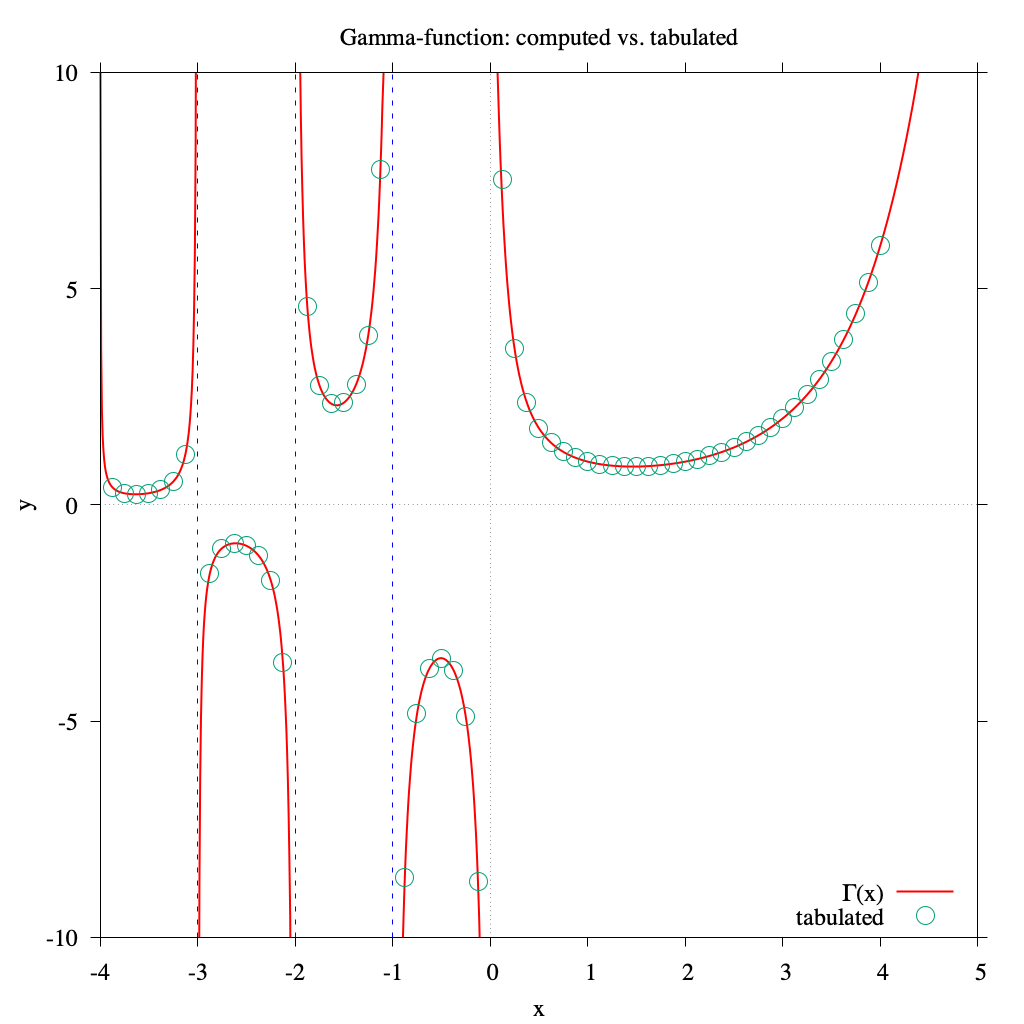
\includegraphics[width=\textwidth]{Plot.png}
    \caption{\textit{The Gamma function calculated with C\# along with tabulated values from the implemented Gamma function
in the C language.}}
    \label{fig:Gamma}
\end{figure}


%+++++++++++++++++++++++++++++++++++++++

\begin{thebibliography}{99}

\bibitem{wiki} \emph{Gamma function},  available at
\url{http://en.wikipedia.org/wiki/Gamma_function}.

\end{thebibliography}


\end{document}

